% Created 2019-06-10 Mon 19:33
% Intended LaTeX compiler: lualatex
\documentclass[presentation]{beamer}
\usepackage{polyglossia}
\setmainlanguage[variant=usmax]{english}
\usepackage{fontspec}
\usepackage{microtype}
\usepackage{geometry}
\usepackage{subfiles}
\usepackage{float}
\usepackage[font=small,labelfont=bf,format=hang]{caption}
\usepackage{amsfonts}
\usepackage{amssymb}
\usepackage{mathtools}
\usepackage[shortlabels]{enumitem}
\usepackage{multirow}
\usepackage{tabularx}
\usepackage{hyperref}
\usepackage{tikz}
\usepackage[edges]{forest}
\usepackage{graphicx}
\usepackage{xcolor}
\usepackage{colortbl}
\usepackage{array}
\usepackage{listings}
\usepackage[autostyle,strict,autopunct]{csquotes}
\usepackage[style=ieee,backend=biber]{biblatex}
\usepackage{tikz}
\usepackage[subpreambles=true]{standalone}
\usepackage{adjustbox}
\usetheme{metropolis}
\author{Eivind D. Halderaker, Sondre Å. Nilsen}
\date{Spring 2019}
\title{INF219 --- MOCCA Operational Controller for Coffee Availability}
\hypersetup{
 colorlinks=true,
 pdfauthor={Eivind D. Halderaker, Sondre Å. Nilsen},
 pdftitle={INF219 --- MOCCA Operational Controller for Coffee Availability},
 pdfkeywords={},
 pdfsubject={},
 pdfcreator={Emacs 26.2 (Org mode 9.2)},
 pdflang={English}}
\begin{document}

\maketitle
\begin{frame}{Plan}
\tableofcontents
\end{frame}


\section{Introduction}
\label{sec:org04b36c4}
\begin{frame}[label={sec:org2b19192}]{Introduction}
\begin{itemize}
\item Coffee is essential to students
\item Therefore knowing if it is ready is vital
\item We have a solution: \emph{MOCCA}
\end{itemize}
\end{frame}
\begin{frame}[label={sec:org1cd23e1}]{The problem}
\begin{figure}[htbp]
\centering
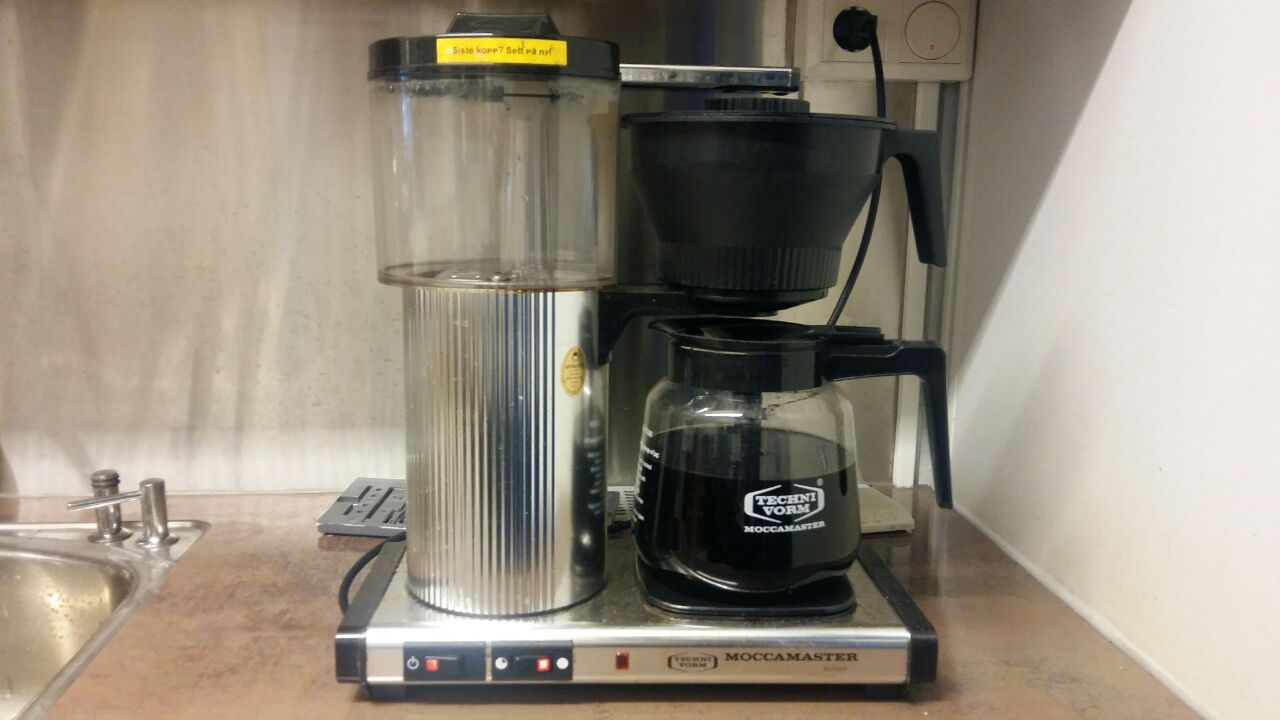
\includegraphics[width=0.7\textwidth]{./figures/brewer.jpeg}
\caption{\label{fix:brewer}
Our drip coffee brewer}
\end{figure}
\end{frame}
\section{System overview}
\label{sec:orgd16040a}
\begin{frame}[label={sec:orgc68645a}]{System overview}
\begin{adjustbox}{max totalsize={.9\textwidth}{.7\textheight},center}
  \documentclass[border=3mm]{standalone}
\usepackage{tikz}
\usetikzlibrary{positioning,fit,arrows.meta,backgrounds}

\tikzset{
  module/.style={%
    draw, rounded corners,
    minimum width=#1,
    minimum height=7mm,
    font=\sffamily
  },
  module/.default=2cm,
  container/.style={
    draw, rounded corners,
    minimum-width=#1,
    minimum height=5cm,
    font=\sffamily
  },
  container/.default=2cm,
  small/.style={
    draw, rounded corners,
    minimum height=2.5cm
    font=\sffamily
  },
  >=LaTeX
}

\begin{document}
\begin{tikzpicture}[->]
  % Arduino box
  \node[module] (Read) {Read from sensors};
  \node[module, below left=1cm and -1cm of Read] (Temp) {Temperature};
  \node[module, below right=1cm and -1cm of Read] (Power) {Power draw};
  \node[small,fit=(Read) (Temp) (Power), draw, label={Arduino}] (SensorBox) {};
  \draw[->] (Read)--(Temp);
  \draw[->] (Read)--(Power);
  % Raspberry Pi processing box
  \node[module, right=2cm of Read] (Camera) {Take picture};
  \node[module, below=of Camera] (CamProcess) {Process};
  \node[small, fit=(Camera) (CamProcess), draw, label={Raspberry Pi}] (Pi2Box) {};
  \draw[->] (Camera)--(CamProcess);
  % Data collection box
  \node[container, fit=(SensorBox) (Pi2Box) (Loop),
  draw, inner xsep=2mm, inner ysep=.5cm,
  label={Data collection}] (DataCollectionBox) {};

  % Data processing box
  \node[module, above right=-1.15cm and 2cm of DataCollectionBox] (AsyncLoop) {Async loop};
  \node[module, below=of AsyncLoop] (Data) {Data processing};
  \node[module, below=of Data] (Storage) {Storage};
  \node[container, fit={(AsyncLoop) (Data) (Storage)},
        draw, inner sep=2mm,
        label={Data processing}]
        (MainBox) {};
  \draw[->] (AsyncLoop)--(Data);
  \draw[->] (Data)--(Storage);

  % Connect main loop and async loop
  \draw[<->] (DataCollectionBox)--(MainBox);

  % Serve box
  \node[module, right=2cm of {AsyncLoop-|MainBox.east}] (Server) {Server};
  \node[module, below=of Server] (API) {API};
  \node[module, below=of API] (Website) {Website};
  \node[container, fit={(Server) (API) (Website)}, draw, inner sep=2mm, label={Serving}] (ServeBox) {};
  \draw[->] (Server)--(API);
  \path[] (Server) edge[bend left=52.5] node [left] {} (Website);
  \draw[->] (API)--(Website);
  \draw[->] (MainBox)--(ServeBox);
\end{tikzpicture}
\end{document}
%%% Local Variables:
%%% mode: latex
%%% TeX-master: t
%%% End:

\end{adjustbox}
\end{frame}
\begin{frame}[label={sec:orgf54014d}]{Data collection}
\begin{block}{Arduino}
Reads temperature and current from brewer
\end{block}
\begin{block}{Raspberry Pi}
Takes a photo of the coffee carafe
\end{block}
\end{frame}
\begin{frame}[label={sec:orgdc2ba15}]{Data collection, sensors}
\begin{center}
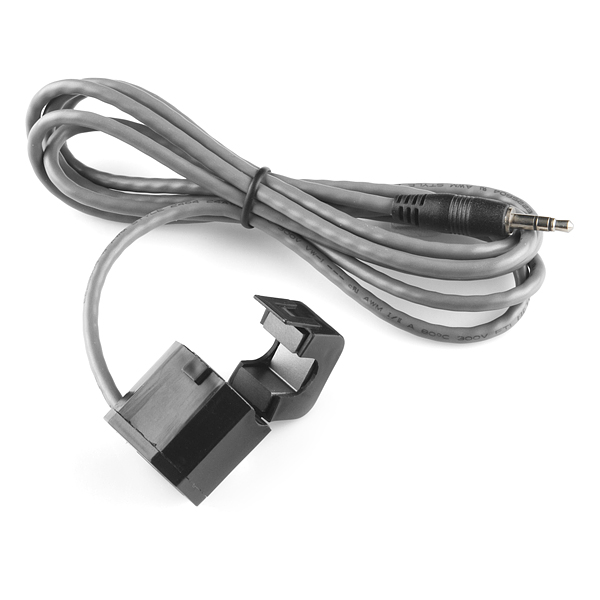
\includegraphics[height=0.3\textwidth]{./figures/currentSensor.jpg}
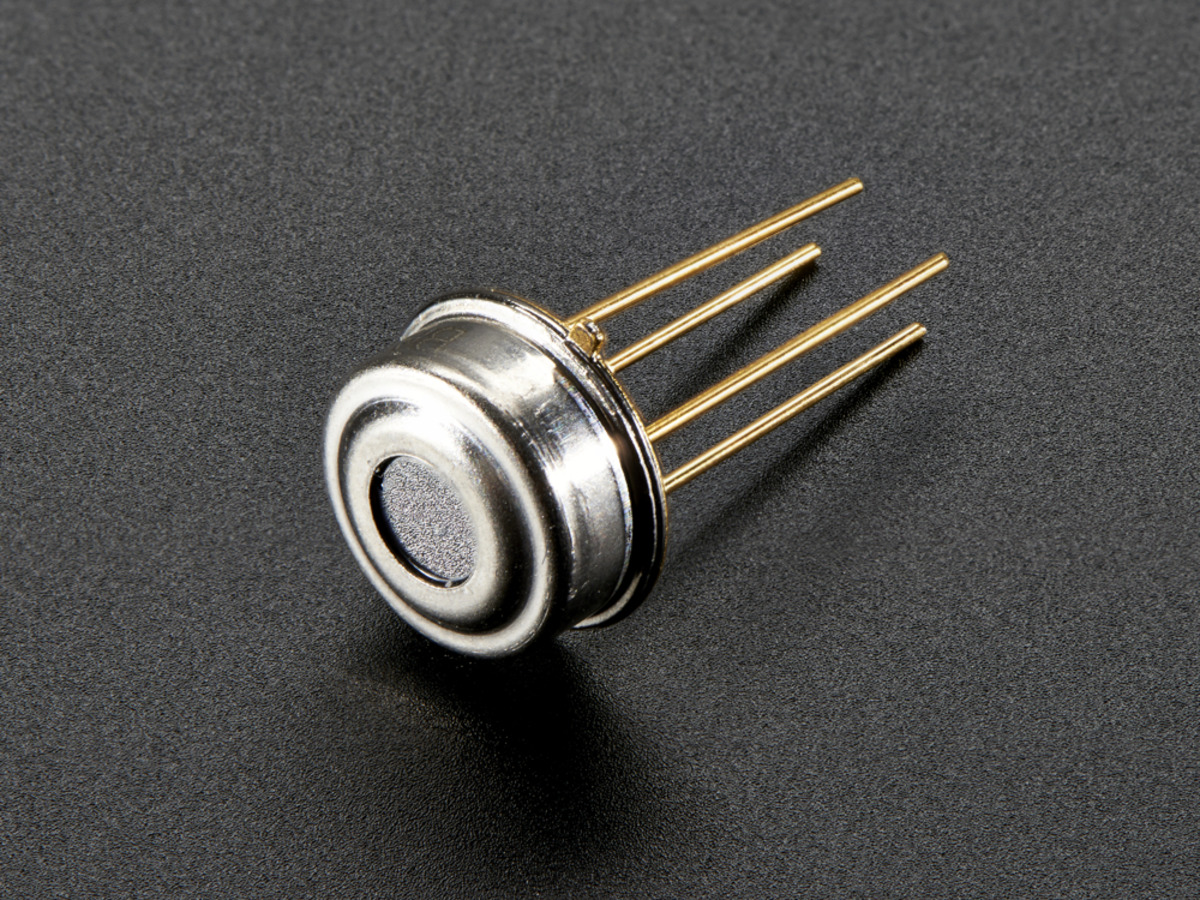
\includegraphics[height=0.3\textwidth]{./figures/tempSensor.jpg}
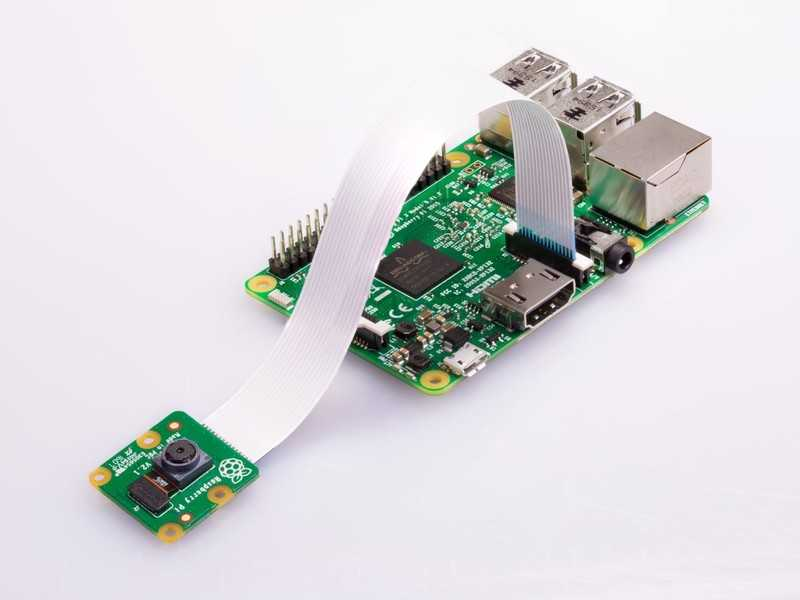
\includegraphics[height=0.3\textwidth]{./figures/cameraSensor.jpg}
\end{center}
\end{frame}
\begin{frame}[label={sec:org368bbef}]{Data processing}
\begin{itemize}
\item Does the heavy lifting
\item Converts raw data to usable data
\end{itemize}
\end{frame}
\begin{frame}[label={sec:orgf130f2d}]{Data processing}
\begin{itemize}
\item Is our interface to the real world
\item Needs to be able to distinguish between fact and fiction
\end{itemize}
\end{frame}
\begin{frame}[label={sec:orgbb14f24}]{Data processing, example}
\begin{figure}[htbp]
\centering
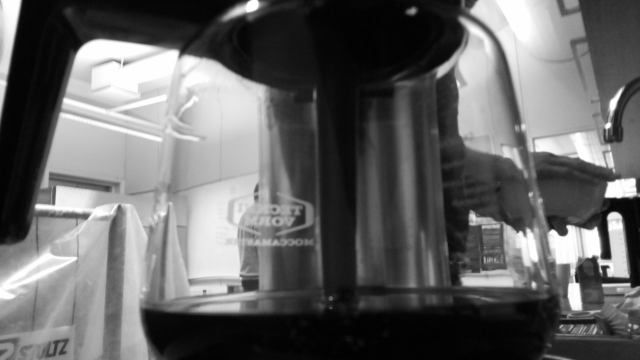
\includegraphics[width=.9\linewidth]{./figures/inputImage.png}
\caption{\label{fig:input-image}
Input image}
\end{figure}
\end{frame}
\begin{frame}[label={sec:org9cdae1f},fragile]{Data processing, example}
 \lstset{frame=tb,columns=fullflexible,flexiblecolumns=true,numbers=left,numberstyle=\ttfamily\color{gray}\tiny,showstringspaces=false,basicstyle=\ttfamily\footnotesize,language=Python,label= ,caption={Image converted to matrix of brightness},captionpos=b}
\begin{lstlisting}
array([[189, 229, 249, ...,  46,  46,  43],
         [179, 221, 246, ...,  47,  44,  43],
         [179, 209, 242, ...,  46,  48,  46],
         ...,
         [135, 140, 141, ...,  41,  43,  41],
         [138, 141, 143, ...,  42,  40,  40],
         [140, 140, 142, ...,  39,  42,  41]], dtype=uint8)
\end{lstlisting}
\end{frame}
\begin{frame}[label={sec:org1692785},fragile]{Data processing, example}
 \lstset{frame=tb,columns=fullflexible,flexiblecolumns=true,numbers=left,numberstyle=\ttfamily\color{gray}\tiny,showstringspaces=false,basicstyle=\ttfamily\footnotesize,language=Python,label= ,caption={Matrix converted to boolean values based on brightness threshold},captionpos=b}
\begin{lstlisting}
array([False, False, False, False, False, False, False,
         False, False, False, False, False, False, False,
         False, False, False, False, False, False, False,
         False, False, False, False, False, False, False,
         False, False, False, False, False, False, False,
         False, False, False, False, False,  True,  True,
         True,  True,  True,  True,  True,  True,  True,
         True,  True,  True,  True,  True,  True,  True,
         True,  True,  True,  True,  True,  True,  True,
         ...,
         False, False, False, False, False, False, False,
         False, False, False, False, False, False, False])
\end{lstlisting}
\end{frame}
\begin{frame}[label={sec:org9e8baa4}]{Data processing, example}
\begin{figure}[htbp]
\centering
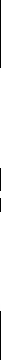
\includegraphics[height=0.5\textwidth]{./figures/outputImage.png}
\caption{\label{fig:output-image}
Output image}
\end{figure}
\end{frame}
\begin{frame}[label={sec:org9f98b01}]{Data serving}
\begin{block}{Back-end}
Serves a REST API that is consumable by applications
\end{block}
\begin{block}{Front-end}
A React web application that shows the current state of the coffee
\end{block}
\end{frame}
\begin{frame}[label={sec:org38b9286}]{Data serving}
\begin{figure}[htbp]
\centering

\includegraphics[width=0.9\textwidth]{./figures/nopower.png}
\caption{\label{fig:no-power}
When the brewer has no power}
\end{figure}
\end{frame}
\begin{frame}[label={sec:org06adcfe}]{Data serving}
\begin{figure}[htbp]
\centering
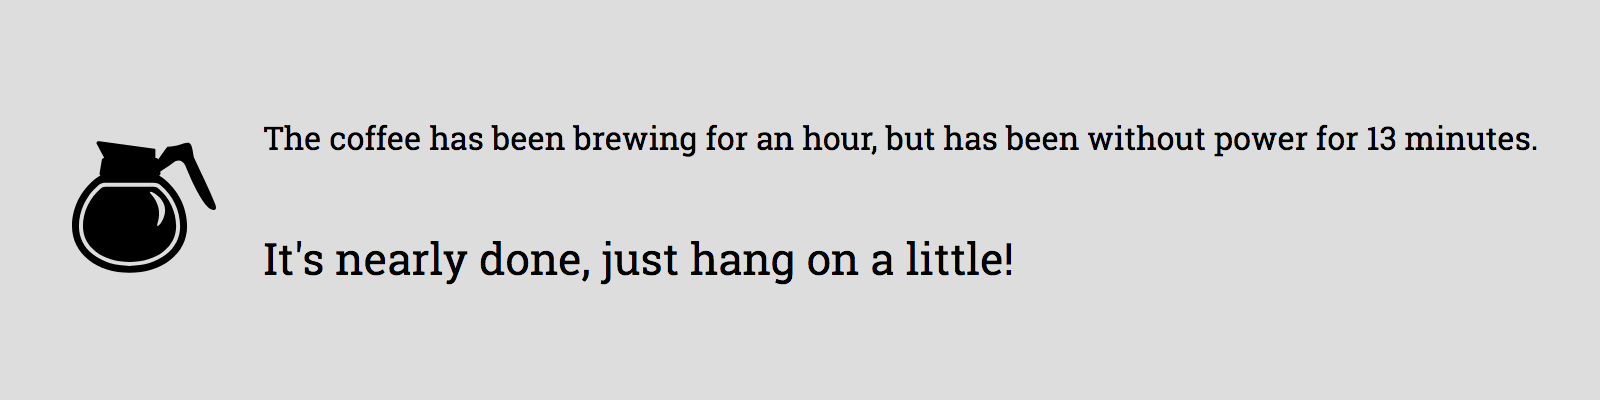
\includegraphics[width=0.9\textwidth]{./figures/brewing.png}
\caption{\label{fig:brewing}
When the coffee is brewing}
\end{figure}
\end{frame}
\section{Conclusion}
\label{sec:org672fb29}
\begin{frame}[label={sec:orge03c030}]{Conclusion}
\begin{itemize}
\item We have created a system that successfully monitors the coffee
\item This is done through a series of subsystems
\item The data is available to anyone willing to use it
\end{itemize}
\end{frame}
\section{Future work}
\label{sec:orgaae0d36}
\begin{frame}[label={sec:orgfb07108}]{Future work}
\begin{itemize}
\item Creating a proper case for the system
\item More historical data available through API
\item A scanner for tracking student coffee consumption
\item Tracking how much coffee is consumed each day
\end{itemize}
\end{frame}
\section{Live demo}
\label{sec:org71b2209}
\end{document}
